\documentclass[12pt]{article}
\usepackage{geometry}
\geometry{a4paper, total={170mm,257mm},left=20mm, top=10mm,}
\usepackage[colorlinks=true,linkcolor=blue,urlcolor=black]{hyperref}
\usepackage{bookmark}
\usepackage{pdfpages}
\begin{document}
\title {Labtainer Student Guide}
\maketitle

\section {Introduction}
This manual is intended for use by students performing labs with Labtainers.
Labtainers assume you have a Linux system, e.g., a virtual machine.  If you
do not have a Linux sysetm, refer to
Appendix A and B for installation of VirtualBox and a Linux system on either
a Mac or a Windows computer.
Note that any Linux system can be used as long as it supports Docker.

Labtainers provide a consistent execution environment for performing
laboratory exercises, and can simulate the execution of several different
computers interconnected via virtual networks.   

\subsection{Obtaining Labtainers and installing Docker}
The Labtainer framework is distributed as a tarball from:
\url{https://my.nps.edu/web/cisr/labtainers}
Click the link named: "Download the Labtainer framework, and untar the resulting file into 
a permanent directory on your Linux system, e.g., into \verb ~/home.  For example, if you downloaded the file
from a browser on your Linux system:
\begin{verbatim}
   cd
   tar -xf ~/Downloads/labtainer.tar
\end{verbatim}
From the directory into which you untarred the
tarball:
\begin{verbatim}
   cd labtainer
   ./install-labtainer.sh
\end{verbatim}

This script will install the latest version of Docker and packages required
by the Labtainer framework.  It will cause your Linux host to reboot when it
completes.
Note that older Linux distributions, e.g., Ubuntu 14.* lack the
\textit{realpath} package, which should be installed prior to using Labtainers.

After the Linux host reboots, open a terminal to your Linux host and
change directory to wherever you untarred the tarball.

\section{Performing a Lab}
All labs are run from the same Labtainer workspace directory:
\begin{verbatim}
    cd labtainer/labtainer-student
\end{verbatim}
\noindent Then run the lab:
\begin{verbatim}
    ./start.py <labname>
\end{verbatim}
\noindent where \textit{labname} is the name of the lab to run.  Leaving this out will 
display a list of available labs.  

Most labs create one or more virtual terminals, one of which may be titled "INSTRUCTIONS".
Please note that some of the initial lab instructions repeat the steps you've already taken, and you need
not perform those again.  Some labs direct you to a PDF version of a lab manual, which can usually 
be done by right clicking on the displayed path, or you can open the file in a browser.

While running the lab, if you require more virtual terminals, use:
\begin{verbatim}
    ./moreterm.py <labname> <container>
\end{verbatim}
\noindent where \textit{container} is the host name of the component on which to attach a terminal.  
It can be omitted for labs having a single component.

The virtual terminals for most labs present bash shells via which you can interact
with the attached computer, (which is actually a Docker container designed to appear
like a separate computer).  A single computer
may have multiple virtual terminals attached to it.  Each computer is independent, and 
may use networks to interact with other Labtainer computers within the lab.  

Many labs automatically gather results of your work, which you will provide to your instructor.
Note that, unless otherwise directed, exploration and experimentation you perform either before
or after performing the expected activity will not diminish or dilute your results.  And you typically
do not have to take actions to collect or record your results.  This occurs automatically as noted in the 
next section.  

\subsection{Stopping Labtainers}
When you are finished, or wish to stop working, type:
\begin{verbatim}
    ./stop.py <labname>
\end{verbatim}
\noindent The stop.py command will display the directory containing a zip file that should be provided to your instructor.
\subsection{Networking}
In addition to network properties defined for the lab,
each component \texttt{/etc/host} file includes a "my\_host entry" that names
the host Linux.  Most containers will include a default gateway that
leads to the Linux host.  This allows students to scp files to/from the container and host.
It also allows the student to reach external networks, e.g., to fetch additional packages in
support of student exploration.

In some instances, the lab requires one or more components to a have different default route.
Typically, these components will include a \textit{togglegw.sh} script that the student
can use to toggle the default gateway between one that leads to the host, and one defined for the lab.
This allows students to add packages on components having lab-specific default gateways.
Use of the \textit{togglegw.sh} script is not necessary to reach the Linux host, (e.g., to scp files).

\subsection{Installing and Using Labtainer Behind a Proxy}
If you are behind a proxy, e.g., in a corporate environment, Labatiner installation
requires that you have configured your Linux package management configuration to reflect
the proxy, e.g., the /etc/atp/apt.conf or /etc/dnf.conf files.  Additionally,
you will need to configure your Docker service as described at:
\url{https://docs.docker.com/engine/admin/systemd/#httphttps-proxy}
And set the HTTP\_PROXY environment variable to your proxy, e.g., 
\begin{verbatim}
HTTP_PROXY=http://myproxy:3128
\end{verbatim}
If you wish to use apt-get from within a container to add new software to a container, you
must first modify the container's /etc/apt/apt.conf file to reflect your proxy.

\subsection{Limitations}
The Labtainer "computers" are individual Docker containers that are interconnected via virtual
networks.  These containers each share the Linux kernel of your host.  Thus, a change
to the kernel configuration on one computer, (e.g., enabling ASLR), will be visible on
other containers, as well as your host.

The computers each include a ".local" directory beneath the HOME directory.  This is used
by the Labtainer framework and includes results that get packaged up for forwarding to the
instructor.  Do not modify any files beneath the .local directory.  Otherwise, you can treat
those containers as Linux systems, and explore them.

Please note that while running some programs in the Labtainer computers, passwords provided to
applications such as "ssh" are not suppressed.  This is a side effect of the Labtainer
support for automated assessment.  

Pasting multiple commands into a labtainer terminal may result in the not all of the
commands being executed.


\appendix 
\section {Appendix A: Installing Virtual Box and Ubuntu on a Mac}
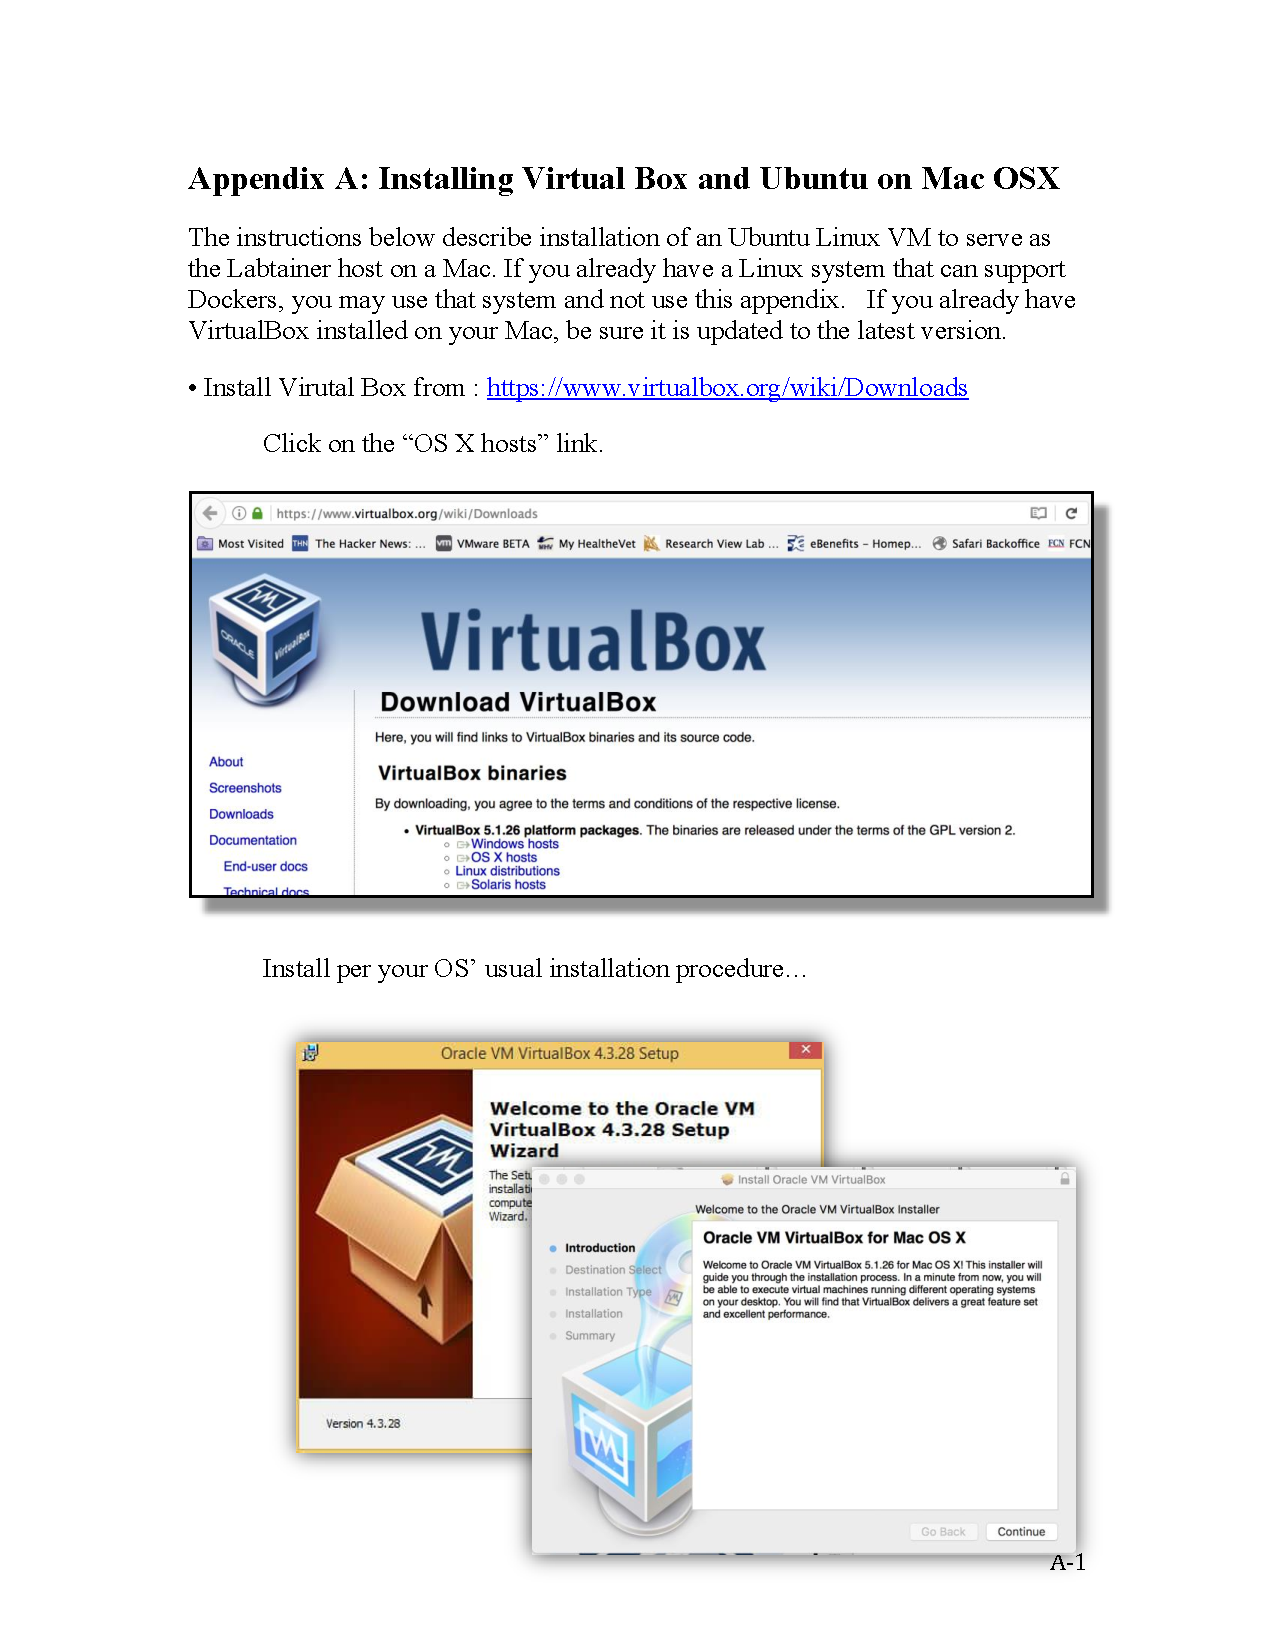
\includepdf[pages=-]{InstallingVB-LinuxMac.pdf}
\appendix 
\section {Appendix B: Installing Virtual Box and Ubuntu on Windows}
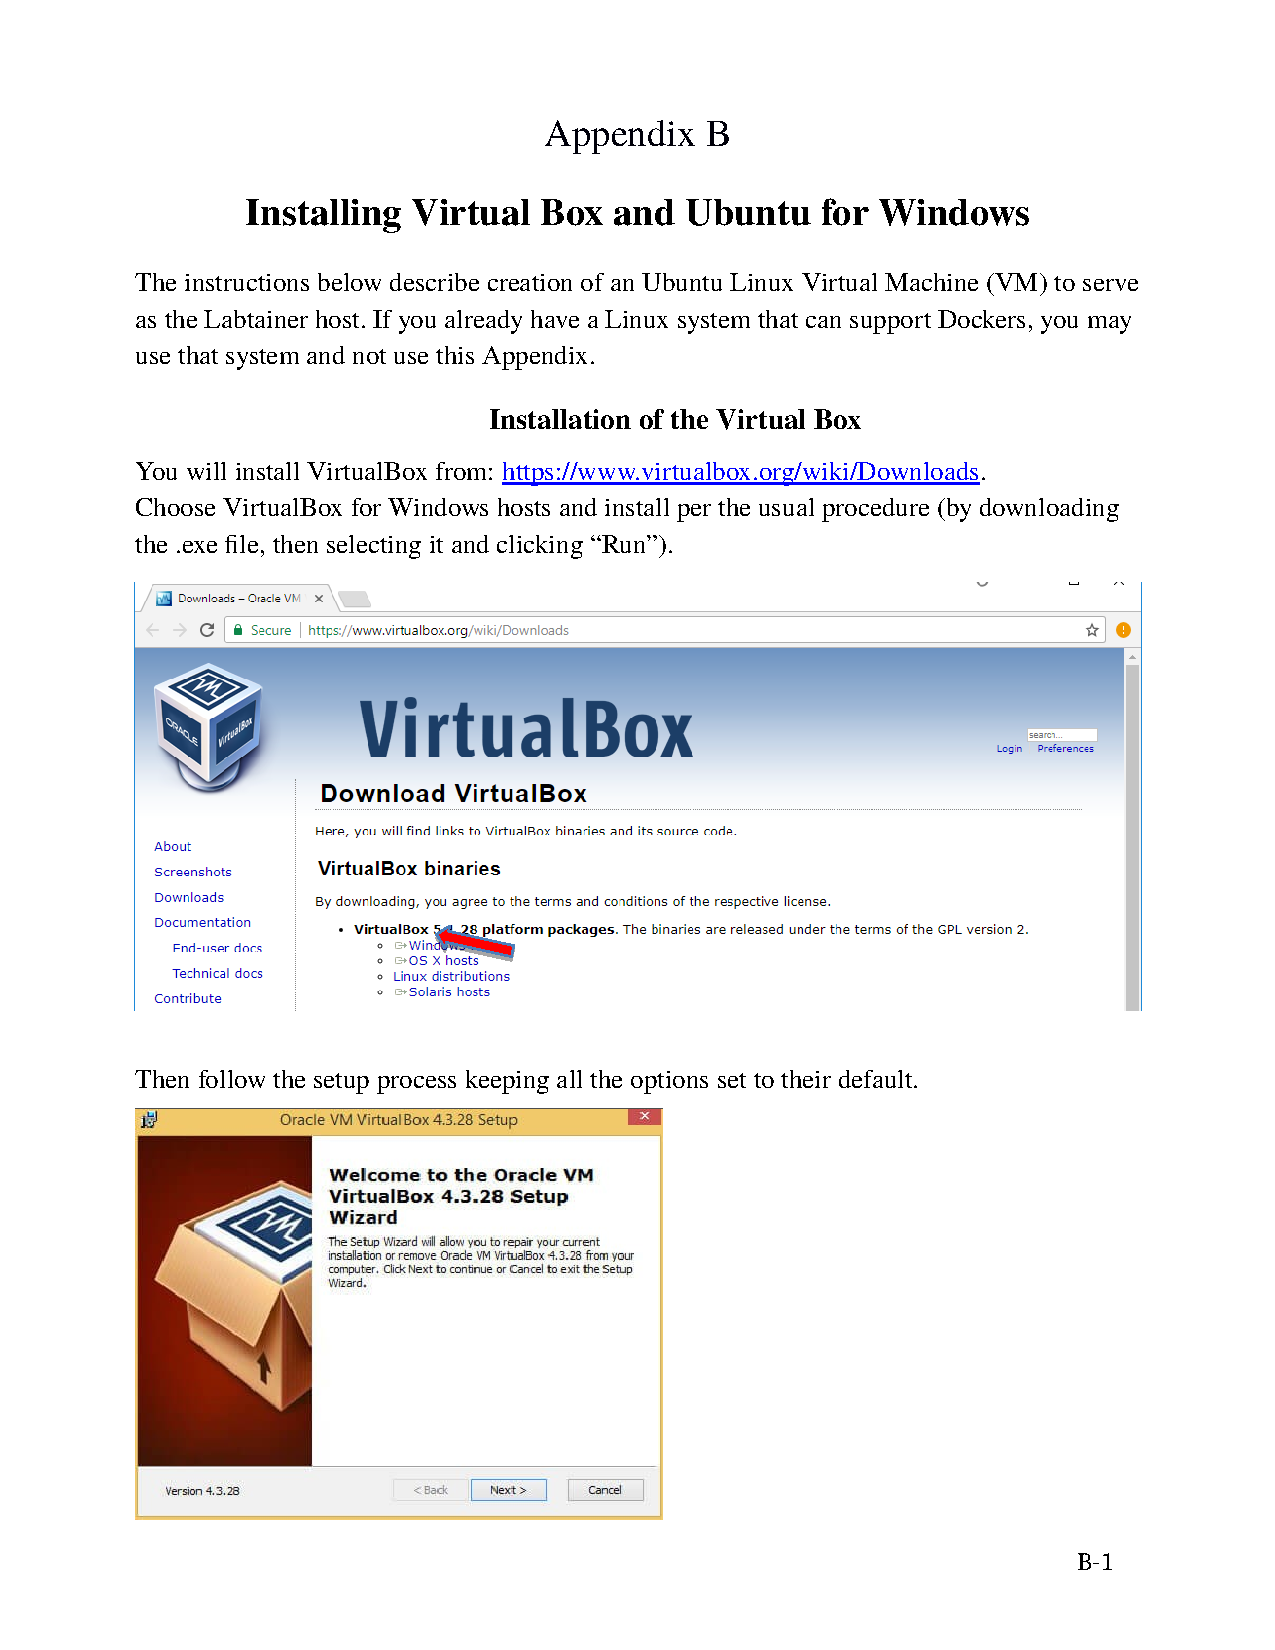
\includepdf[pages=-]{InstallingVB-LinuxWin.pdf}
\appendix 
\section {Appendix C: Labtainer Command Summary}
\label{sec:appendixC}
The following labtainer commands are available from the \texttt{labtainer/labtainer-student}
directory:
\begin{itemize}
\item \texttt{./start.py <lab> --}
Start the named lab.  If no name is given, a list of available labs will be displayed.
\item \texttt{./stop.py <lab> --} Stop the named lab.
\item \texttt{./moreterm.py <lab> <container> --} create a new virtual terminal for the container.
\item \texttt{./redo.py <lab> --}
Delete any previous containers associated with this lab and start it fresh.  \textbf{Warning}: this will lose any
previous data from the named lab.
\end{itemize}

Most labs display lab instructions in one of the windows that appears after the lab starts.  If those instructions
stop displaying, e.g., because "q" is pressed in that window, then type the following in a virtual terminal (e.g.,
in a new terminal created using the ./moreterm.py script:
\begin{verbatim}
    less instructions.txt
\end{verbatim}


\end{document}
